%This is a LaTeX template for homework assignments
\documentclass[8pt]{article}
\usepackage[top=1in, bottom=1in, left=1.1in, right=1.1in]{geometry}
\usepackage[utf8]{inputenc}
\usepackage{amsmath}
\usepackage{CJK}
\usepackage{enumerate}
\usepackage{ifthen}
\usepackage{listings}
\lstset{
  language=python,
  keywordstyle=\color{blue!70},
  frame=single,
  basicstyle=\ttfamily,
  commentstyle=\color{red},
  breakindent=0pt,
  rulesepcolor=\color{red!20!green!20!blue!20},
  rulecolor=\color{black},
  tabsize=4,
  numbersep=5pt,
  showstringspaces=false,
  breaklines=true,
  backgroundcolor=\color{red!10},
  showspaces=false,
  showtabs=false,
  extendedchars=false,
  escapeinside=``,
  frame=no,
}

\usepackage{fourier}
\usepackage{pgf}
\usepackage{tikz}
\usetikzlibrary{calc}
\usetikzlibrary{arrows,snakes,backgrounds,shapes,shadows}
\usetikzlibrary{matrix,fit,positioning,decorations.pathmorphing}



\newcommand{\tf}{\ttfamily}


\newlength{\la}
\newlength{\lb}
\newlength{\lc}
\newlength{\ld}
\newlength{\lhalf}
\newlength{\lquarter}
\newlength{\lmax}
\newcommand{\xx}[4]{\\[.5pt]%
\settowidth{\la}{A.~#1~~}
\settowidth{\lb}{B.~#2~~}
\settowidth{\lc}{C.~#3~~}
\settowidth{\ld}{D.~#4~~}
%%
\ifthenelse{\lengthtest{\la>\lb}}
{\setlength{\lmax}{\la}}
{\setlength{\lmax}{\lb}}
\ifthenelse{\lengthtest{\lmax<\lc}}
{\setlength{\lmax}{\lc}}
{}
\ifthenelse{\lengthtest{\lmax<\ld}}
{\setlength{\lmax}{\ld}}
{}
%%
\setlength{\lhalf}{0.5\linewidth}
\setlength{\lquarter}{0.25\linewidth}
%%
\ifthenelse{\lengthtest{\lmax>\lhalf}}
{\noindent{}A.~#1 \\ B.~#2 \\ C.~#3 \\ D.~#4 }
{
\ifthenelse{\lengthtest{\lmax>\lquarter}}
{\noindent
\makebox[\lhalf][l]{A.~#1~~}%
\makebox[\lhalf][l]{B.~#2~~}\\
\makebox[\lhalf][l]{C.~#3~~}%
\makebox[\lhalf][l]{D.~#4~~}
}%
{\noindent
\makebox[\lquarter][l]{A.~#1~~}%
\makebox[\lquarter][l]{B.~#2~~}%
\makebox[\lquarter][l]{C.~#3~~}%
\makebox[\lquarter][l]{D.~#4~~}
}
}
}



\begin{document}
\begin{CJK}{UTF8}{gkai}
\begin{center}
{\Large \bf  武汉大学数学与统计学院2017-2018学年第一学期期末考试\\[0.1in]
  数据结构与算法(A卷答案)} \vspace{0.1in}

\end{center}


\begin{enumerate} %\line(1,0){20}
\item (20分)~Python相关
  \begin{enumerate}
  \item (5分)
    \begin{lstlisting}
dict = {'Name':'Li Ming', 'Sex':'Male', 
        'HomeTown':'Wuhan', 'Age':20}
    \end{lstlisting}
    \begin{lstlisting}
set = {2, 'Python', True, 3.14}
     \end{lstlisting}
  \item (5分)
    \begin{lstlisting}
[0, 1, 2, 3, 4, 5, 6, 7, 8, 9]
[10, 11, 12, 13, 14, 15, 16, 17, 18, 19]
[0, 2, 4, 6, 8]
[0, 2, 4, 6, 8, 10, 12, 14, 16, 18]
    \end{lstlisting}
  \item (5分)
\begin{lstlisting}
alist = [x * x for x in range(1, 11) if x % 2 == 0]
  \end{lstlisting}
  \begin{lstlisting}
alist = [m + n for m in 'abc' for n in '1234']
  \end{lstlisting}
\item (5分)
  \begin{lstlisting}
class Rectangle(object):
    def __init__(self, length, width):
        self.length = length
        self.width  = width
    def area(self):
        return self.length *  self.width
    def circum(self):
        return 2 * (self.length + self.width)
  \end{lstlisting}    
  \end{enumerate}
\item (15分)~
  \begin{enumerate}
    \item (6分)
      \begin{lstlisting}
        return self.next
        self.data = newdata
        self.next = newnext
      \end{lstlisting}
    \item (9分)
      \begin{lstlisting}
        Node(item)
        self.head
        self.head = temp

        current != None and not found:
        current.getData() == item:
        current = current.getNext()
       

        previous = current
        current = current.getNext()
        self.head = current.getNext()
      \end{lstlisting}
  \end{enumerate}
\item (15分)
  \begin{enumerate}
    \item (6分)
      \begin{lstlisting}
        self.items.append(item)
        return self.items.pop()
        return self.items[len(self.items)-1]
      \end{lstlisting}
    \item (9分)
      \begin{lstlisting}
        stack.push(rem)
        not stack.isEmpty():
        binString = binString + str(stack.pop())
      \end{lstlisting}
  \end{enumerate}
\item (20分)~队列与二叉树
  \begin{enumerate}
  \item (4分)~
    \begin{lstlisting}
      self.items.insert(0, item)
      return self.items.pop()
    \end{lstlisting}
  \item (4分)~
    \begin{lstlisting}
      self.lchild = BinaryTree(newNode)
      t = BinaryTree(newNode)
      t.lchild = self.lchild
      self.lchild = t
      \end{lstlisting}
      
  \item (4分)
    \begin{lstlisting}
      tree
      inorder(tree.getLeftChild())
      print(tree.getRootVal())
      inorder(tree.getRightChild())
    \end{lstlisting}
  \item (4分)
    \begin{lstlisting}      
      q.enqueue(node)
      node = q.dequeue()
      q.enquque(node.lchild)
      q.enqueue(node.rchild)    
    \end{lstlisting}
  \item (4分)
    \begin{figure}[htbp]
      \centering
    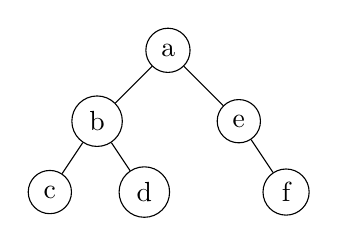
\begin{tikzpicture}[scale=0.6]
      \tikzstyle{every node}=[circle,draw]
      \tikzstyle{level 1}=[sibling distance=3cm]
      \tikzstyle{level 2}=[sibling distance=2cm]
      \node at (0,0) {a} 
      child {node{b} child {node{c}} child {node{d}}} 
      child {node{e} child [fill=none] {edge from parent[draw=none]} child {node{f}} };
    \end{tikzpicture}
  \end{figure}
  \begin{lstlisting}
tree = BinaryTree('a')
tree.insertLeft('b')
tree.insertRight('e')   
tree.getLeftChild().insertLeft('c')
tree.getLeftChild().insertRight('d')
tree.getRightChild().insertRight('f')

inorder(tree)
levelorder(tree)
\end{lstlisting}

\begin{lstlisting}[title=运行结果]
cbdaef
abecdf
\end{lstlisting}
  \end{enumerate}
\item (15分)~ 
  \begin{enumerate}
  \item (5分)~
    \begin{lstlisting}
def sequentialSearch(alist, item):
    pos = 0
    found = False
    while pos < len(alist) and not found:
        if alist[pos] == item:
            return True
        else:
            pos = pos + 1
    return found
    \end{lstlisting}
  \item (5分)~
    \begin{lstlisting}
def mergeSort(alist):
    if len(alist) > 1:
        mid = len(alist) // 2
        left = alist[:mid]
        right = alist[mid:]

        mergeSort(left)
        mergeSort(right)

        i = 0
        j = 0 
        k = 0
        while i < len(left) and j < len(right):
            if left[i] < right[i]:
                alsit[k] = left[i]
                i += 1
            else:
                alist[k] = right[j]
                j += 1
        k += 1

        while i < len(left):
            alist[k] = left[i]
            i += 1
            k += 1

        while j < len(right):
            alist[k] = right[j]
            j += 1
            k += 1
    \end{lstlisting}
  \item (5分)~
    \begin{lstlisting}
alist = [53, 24, 91, 88, 34, 71, 44, 18]

if sequentialSearch(alist, 88):
    print('Exist!')
else:
    print('Failed!')

print(alist)
mergeSort(alist)
print(alist)
    \end{lstlisting}
  \end{enumerate}
\item (15分)~
  \begin{figure}[htbp]
    \centering
  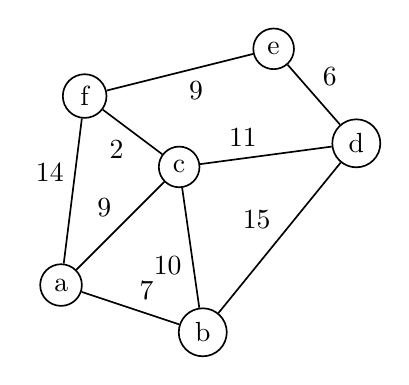
\begin{tikzpicture}[scale=1.5,node distance=3cm,semithick,inner sep=3pt,bend angle=45,auto]
    % \draw[help lines] (0,-1) grid (7,3);
    \node[circle,draw]   (a) at (0,0)  {a};
    \node[circle,draw]   (b) at (1.2,-.4)   {b};
    \node[circle,draw]   (c) at (1.0,1.0) {c};
    \node[circle,draw]   (d) at (2.5,1.2){d};
    \node[circle,draw]   (e) at (1.8,2.0){e};
    \node[circle,draw]   (f) at (0.2,1.6){f};
    \path
    (a) edge node{ 7}      (b)
        edge node{ 9}      (c)
        edge node{14}      (f)
    (b) edge node{10}      (c)
        edge node{15}      (d)
    (c) edge node{ 2}      (f)
        edge node{11}      (d)
    (e) edge node{ 9}      (f)
        edge node{ 6}      (d);
  \end{tikzpicture}
\end{figure}
\begin{enumerate}
  \item (5分)
    \begin{figure}[htbp]
      \centering
      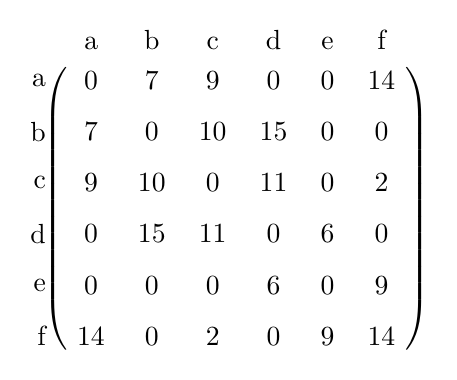
\begin{tikzpicture}[scale=1.5,node distance=3cm,semithick,inner sep=1pt,bend angle=45,auto]
        \matrix (am)  [matrix of math nodes,left delimiter=(,right delimiter=),row sep=10pt,column sep=10pt,right] 
        {
          0 & 7 & 9 & 0 & 0 &14\\
          7 & 0 &10 &15 & 0 & 0\\
          9 & 10& 0 &11 & 0 & 2\\
          0 & 15&11 & 0 & 6 & 0\\
          0 & 0 & 0 & 6 & 0 & 9\\
          14& 0 & 2 & 0 & 9 &14\\
        };
        \node at (am-1-1) [above=10pt] {a}; 
        \node at (am-1-2) [above=10pt] {b};       
        \node at (am-1-3) [above=10pt] {c};       
        \node at (am-1-4) [above=10pt] {d};
        \node at (am-1-5) [above=10pt] {e};
        \node at (am-1-6) [above=10pt] {f};
        \node at (am-1-1) [left=15pt] {a}; 
        \node at (am-2-1) [left=15pt] {b};       
        \node at (am-3-1) [left=15pt] {c};       
        \node at (am-4-1) [left=15pt] {d};             
        \node at (am-5-1) [left=15pt] {e};             
        \node at (am-6-1) [left=15pt] {f};             
      \end{tikzpicture}
    \end{figure}
  \item (5分)
    \begin{lstlisting}
{'a': 3, 'b': 3, 'c': 4, 'd': 3, 'e': 2, 'f': 3}     
    \end{lstlisting}
  \item (5分)~
    \begin{lstlisting}[title=深度优先]
a, b, c, d, e, f          
    \end{lstlisting}
    \begin{lstlisting}[title=广度优先]
a, b, c, f, d, e
    \end{lstlisting}

\end{enumerate}
\end{enumerate}



\end{CJK}
\end{document}
